% Snowflake Data Engineering — Chapter 2 | original manuscript draft
% Author: Arman Golbidi | Editorial snapshot: 21 October 2026
% Compile: xelatex -interaction=nonstopmode -halt-on-error Snowflake_Data_Engineering_Chapter_01.tex
% Trim: 178 x 254 mm; margins inside 23 mm / outside 17 mm / top-bottom 19 mm.
% Body: 10.75 pt / 13.65 pt leading = 1.27 line-height ratio; code: 8.75 pt.
\documentclass[11pt,twoside]{article}
\usepackage[paperwidth=178mm,paperheight=254mm,inner=23mm,outer=17mm,top=19mm,bottom=19mm,headheight=5mm,headsep=4mm,footskip=9mm]{geometry}
\usepackage{fontspec}
\setmainfont{LibertinusSerif-Regular.otf}[BoldFont=LibertinusSerif-Bold.otf,ItalicFont=LibertinusSerif-Italic.otf,BoldItalicFont=LibertinusSerif-BoldItalic.otf]
\setsansfont{LibertinusSans-Regular.otf}[BoldFont=LibertinusSans-Bold.otf,ItalicFont=LibertinusSans-Italic.otf]
\setmonofont{LibertinusMono-Regular.otf}[Scale=0.91]
\usepackage[english]{babel}
\usepackage{microtype}
\usepackage{setspace}
\setstretch{1.0}
\usepackage{titlesec,enumitem,tabularx,array,booktabs,needspace,fancyhdr,lastpage}
\usepackage[most]{tcolorbox}
\usepackage{tikz}
\usetikzlibrary{arrows.meta,positioning,fit,shapes.misc,calc}
\usepackage{listings}
\usepackage{xcolor}
\usepackage{hyperref}
\hypersetup{colorlinks=true,urlcolor=steelblue,linkcolor=steelblue,pdfauthor={Arman Golbidi},pdftitle={Snowflake Data Engineering - Chapter 2: Snowflake Architecture: Storage, Compute, and Services},pdfsubject={English technical book manuscript, second chapter, 178 x 254 mm}}
\definecolor{navy}{HTML}{15334A}
\definecolor{steelblue}{HTML}{17779B}
\definecolor{teal}{HTML}{12888A}
\definecolor{lightblue}{HTML}{ECF5F7}
\definecolor{papergray}{HTML}{F2F5F6}
\definecolor{inkgray}{HTML}{4A5862}
\definecolor{thinrule}{HTML}{CBD7DB}
\AtBeginDocument{\color{navy}\fontsize{10.75}{13.65}\selectfont}
\setlength{\parindent}{0pt}
\setlength{\parskip}{3.3pt plus 0.7pt minus 0.6pt}
\setlist[itemize]{leftmargin=4mm,itemsep=1pt,topsep=2pt,parsep=0pt}
\setlist[enumerate]{leftmargin=5mm,itemsep=1pt,topsep=2pt}
\titleformat{\section}{\sffamily\bfseries\color{navy}\fontsize{14}{17}\selectfont}{}{0pt}{}
\titlespacing*{\section}{0pt}{8pt}{4pt}
\titleformat{\subsection}{\sffamily\bfseries\color{steelblue}\fontsize{10.8}{13}\selectfont}{}{0pt}{}
\titlespacing*{\subsection}{0pt}{5pt}{1pt}
\newcommand{\topic}[2]{\subsection*{#1\quad #2}}
\newcommand{\repo}[2]{\par\begingroup\fontsize{8.0}{9.6}\selectfont\sffamily\color{inkgray}\textbf{Project reference:} \href{#2}{#1}. \textit{Not independently executed; rights review pending.}\par\endgroup}
\newtcolorbox{insight}[1][]{enhanced,breakable,colback=lightblue,colframe=thinrule,boxrule=.45pt,arc=1.3mm,left=2.8mm,right=2.8mm,top=1.8mm,bottom=1.8mm,before skip=5pt,after skip=5pt,#1}
\newtcolorbox{whitebox}[1][]{enhanced,breakable,colback=papergray,colframe=thinrule,boxrule=.35pt,arc=1mm,left=2.6mm,right=2.6mm,top=1.5mm,bottom=1.5mm,before skip=4pt,after skip=5pt,#1}
\lstdefinestyle{chaptercode}{basicstyle=\ttfamily\fontsize{8.75}{10.7}\selectfont,backgroundcolor=\color{papergray},frame=single,framerule=.35pt,rulecolor=\color{thinrule},breaklines=true,columns=fullflexible,keepspaces=true,showstringspaces=false,aboveskip=5pt,belowskip=5pt,xleftmargin=2mm,xrightmargin=1mm,framexleftmargin=2mm,framexrightmargin=1mm}
\lstset{style=chaptercode}
\pagestyle{fancy}
\fancyhf{}
\fancyhead[LE]{\sffamily\fontsize{7.6}{9}\selectfont\color{inkgray}\textsc{Snowflake Data Engineering}}
\fancyhead[RO]{\sffamily\fontsize{7.6}{9}\selectfont\color{inkgray}\textsc{02 / Snowflake Architecture}}
\fancyfoot[LE,RO]{\sffamily\bfseries\fontsize{8.2}{9}\selectfont\color{steelblue}\thepage}
\fancyfoot[LO,RE]{\sffamily\fontsize{7.6}{9}\selectfont\color{inkgray}Arman Golbidi \quad | \quad Chapter 02}
\renewcommand{\headrulewidth}{0.35pt}
\renewcommand{\footrulewidth}{0pt}
\setcounter{page}{21}
\raggedbottom

% CHAPTER 02 ONLY, pages 21--38 in the planned book
\begin{document}
% PAGE 21: OPENING
{\sffamily\bfseries\color{teal}\fontsize{10}{12}\selectfont CHAPTER 02\quad /\quad ARCHITECTURE}\par\vspace{2mm}
{\sffamily\bfseries\color{navy}\fontsize{23}{26}\selectfont Snowflake Architecture:\par Storage, Compute,\par and Services}\par
\vspace{1.7mm}{\color{steelblue}\rule{\linewidth}{1.5pt}}\par
\vspace{2mm}{\sffamily\color{inkgray}\fontsize{11.2}{15}\selectfont Follow one query, then decide what to scale.}\par\vspace{2mm}

At 09:01, a Finnish energy analyst opens an hourly-generation report. The query returns in 1.7 seconds. At 09:02, twelve colleagues refresh the same dashboard and several requests wait in a queue. The team could buy a larger warehouse, add compute clusters, change the table's organization, or improve the query. Each response has a different cost and attacks a different bottleneck.

The right choice depends on where the time was spent. Did Snowflake read too many micro-partitions? Was the data cached? Did the request wait for compute? Did an authorization check or compilation dominate? The words \emph{storage}, \emph{compute}, and \emph{cloud services} are useful only when they help answer these questions. This chapter builds a precise mental model of those responsibilities and shows how to inspect evidence before making a change.

\begin{insight}
\textbf{The central question}\par
When a Snowflake workload becomes slow, expensive, or difficult to govern, which architectural layer is responsible---and which change is justified by the evidence?
\end{insight}
\textbf{Learning outcomes.} By the end of the chapter you can:
\begin{itemize}
\item Draw the three-layer architecture and trace an authorized query from request to result.
\item Explain columnar micro-partitions, metadata pruning, and why loading order can matter.
\item Distinguish warehouse resizing, compute isolation, and concurrency scaling.
\item Read a Query Profile without confusing a query-result cache hit with actual execution speed.
\item Describe Time Travel, Fail-safe, retention limits, region dependencies, and table-type decisions.
\item Produce an architecture decision record and a safe, reviewable performance investigation.
\end{itemize}
\textbf{Prerequisites.} Chapter 1 and basic familiarity with \texttt{SELECT}, \texttt{WHERE}, and \texttt{GROUP BY}. The architecture exercise has an offline route. Optional SQL investigation requires an appropriately configured Snowflake account and a low-cost, least-privilege test warehouse.


\newpage
% PAGE 22 - 2.1
\section*{2.1\quad The three architectural layers}
\topic{2.1.1}{Storage, virtual warehouses, and cloud services}
Snowflake's core model separates \emph{persistent data}, \emph{computing resources}, and \emph{coordination services}. It is a managed cloud service, not a package installed on a local server. A table's persistent bytes are managed independently from a virtual warehouse that scans and transforms them. The cloud-services layer maintains much of the coordination required to authenticate a user, resolve metadata, compile a query, and dispatch its plan [1].

\begin{center}
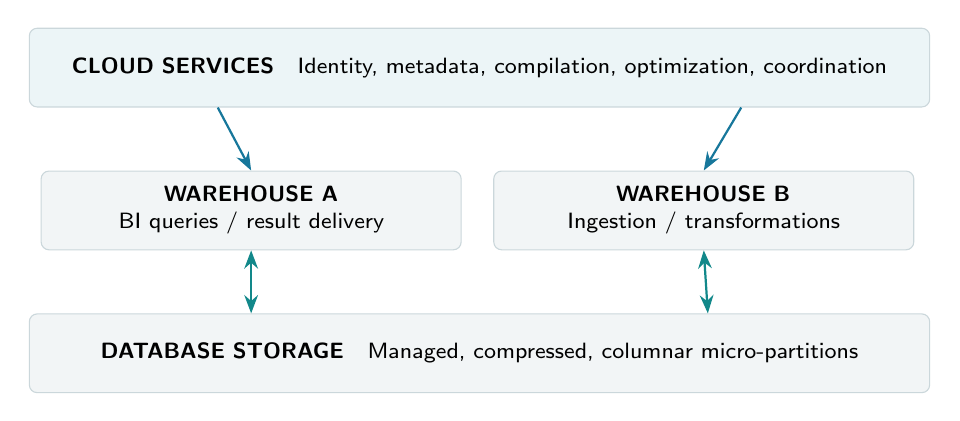
\begin{tikzpicture}[every node/.style={font=\sffamily\fontsize{8}{9.7}\selectfont}, unit/.style={draw=thinrule,fill=papergray,rounded corners=1mm,align=center,minimum height=10mm},>=Stealth]
\node[unit,text width=112mm,fill=lightblue] (svc) {\textbf{CLOUD SERVICES}\quad Identity, metadata, compilation, optimization, coordination};
\node[unit,text width=51mm,below=8mm of svc,xshift=-29mm] (w1) {\textbf{WAREHOUSE A}\\ BI queries / result delivery};
\node[unit,text width=51mm,right=4mm of w1] (w2) {\textbf{WAREHOUSE B}\\ Ingestion / transformations};
\node[unit,text width=112mm,below=8mm of w1,xshift=29mm] (sto) {\textbf{DATABASE STORAGE}\quad Managed, compressed, columnar micro-partitions};
\draw[->,thick,steelblue] (svc.south west) ++(24mm,0)--(w1.north);
\draw[->,thick,steelblue] (svc.south east) ++(-24mm,0)--(w2.north);
\draw[<->,thick,teal] (w1.south)--($(sto.north)+(-29mm,0)$);
\draw[<->,thick,teal] (w2.south)--($(sto.north)+(29mm,0)$);
\end{tikzpicture}
\end{center}
{\small\color{inkgray}\textbf{Figure 2.1.} A conceptual view of Snowflake. The arrows explain responsibility, not private implementation internals or a guaranteed physical data path.}\par

\topic{2.1.2}{Responsibilities and relative isolation}
Separate warehouses can use the same logical tables while having distinct compute resources and billing. This is valuable when a heavy transformation should not contend for the same execution slots as interactive reporting. It does \emph{not} mean that all platform activity is isolated: warehouses still depend on common storage, account governance, metadata, and cloud services. Nor does it mean an idle warehouse can read data without any compute being used by a query; cached-result retrieval is a separate behavior.

\topic{2.1.3}{Tracing a data and command flow}
A simplified \texttt{SELECT} passes through authentication and authorization, object resolution, compilation/optimization, scheduling on a warehouse if execution is needed, columnar scanning and operators, and result delivery. Some requests may reuse an eligible persisted result without rerunning the original work. The important distinction is between \emph{logical steps} and claims about proprietary internal execution order; Figure 2.1 depicts the former [1,5].

\textbf{Decision check.} If dashboard queries queue only when ELT begins, first test separate warehouses; if one filtered query reads most of a large table, inspect pruning before adding compute. \textbf{Failure mode:} concluding that storage and warehouse separation removes every shared dependency.
\repo{P012: Data Engineering with Notebooks}{https://github.com/Snowflake-Labs/sfguide-data-engineering-with-notebooks}

\newpage
% PAGE 23 - 2.2
\section*{2.2\quad Storage organization and micro-partitions}
\topic{2.2.1}{Micro-partitions and metadata}
A standard Snowflake table is not a single row-oriented file. Snowflake stores its data in compressed, columnar micro-partitions and maintains metadata that helps avoid unnecessary reads. The documented typical size is roughly 50--500 MB of \emph{uncompressed} data per micro-partition, not a fixed number of disk bytes. Metadata includes value ranges and distinct-value information that can inform pruning [2]. You do not allocate micro-partitions manually as you might create directories for date partitions in object storage.

\begin{whitebox}
\textbf{Mental model.} A micro-partition is a unit of organized columnar storage with useful statistics. It is not the same as a warehouse, a database schema, an external file, or the partition clause of an Apache Iceberg table.
\end{whitebox}
\topic{2.2.2}{Pruning and load-order effects}
Imagine energy readings loaded in increasing event time. If the timestamp ranges of micro-partitions are relatively narrow, a query for one day may discard many other partitions using metadata. If data for that day is scattered across a large portion of the table, many micro-partitions may overlap the predicate. The load pattern and subsequent changes influence clustering; \emph{there is no guarantee} that chronological ingestion always results in perfect pruning.

\begin{center}
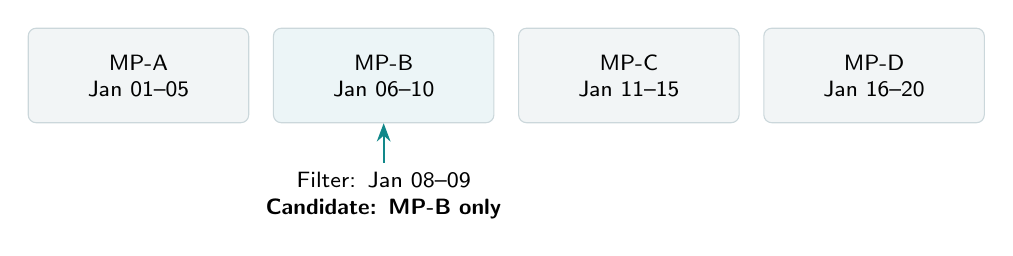
\begin{tikzpicture}[every node/.style={font=\sffamily\fontsize{8}{9.5}\selectfont}, rec/.style={draw=thinrule,minimum width=28mm,minimum height=12mm,rounded corners=1mm,align=center},>=Stealth]
\node[rec,fill=papergray] (a) {MP-A\\ Jan 01--05};
\node[rec,right=3mm of a,fill=lightblue] (b) {MP-B\\ Jan 06--10};
\node[rec,right=3mm of b,fill=papergray] (c) {MP-C\\ Jan 11--15};
\node[rec,right=3mm of c,fill=papergray] (d) {MP-D\\ Jan 16--20};
\node[below=5mm of b,align=center,text width=59mm] (p) {Filter: Jan 08--09\\\textbf{Candidate: MP-B only}};
\draw[->,thick,teal] (p.north)--(b.south);
\end{tikzpicture}
\end{center}
{\small\color{inkgray}\textbf{Figure 2.2.} Illustrative non-overlapping date ranges. Real micro-partition ranges may overlap; the figure is not a measured Query Profile.}\par

\topic{2.2.3}{Compared with manually managed partitions}
Unlike explicitly partitioned files in a data lake, the engineer does not usually write a \texttt{PARTITION BY} scheme for standard Snowflake tables. Instead, concentrate first on data types, selective predicates, load patterns, and observed scans. Clustering keys and automated reclustering are further tools, not automatic prerequisites for every table; maintenance has costs [2].

\textbf{Failure mode.} A filter such as \texttt{DATE(event\_ts) = ...} may be easier to read but should not automatically be assumed to prune like a direct range predicate; compare query plans with your actual data. \textbf{Evidence to seek:} TableScan \emph{Partitions scanned} against \emph{Partitions total} and logical bytes read [6].
\repo{P013: Getting Started with pandas on Snowflake}{https://github.com/Snowflake-Labs/sfguide-getting-started-with-pandas-on-snowflake}

\newpage
% PAGE 24 - 2.3
\section*{2.3\quad Virtual warehouses and compute isolation}
\topic{2.3.1}{Warehouse roles, start/stop, and auto-suspend}
A virtual warehouse supplies compute for many SQL queries and certain processing jobs; it is distinct from the account that owns tables and roles. Assign different virtual warehouses to different workloads where isolation matters. A warehouse can be started, resized, and suspended. \texttt{AUTO\_SUSPEND} and \texttt{AUTO\_RESUME} help avoid leaving test compute active, but do not remove storage, cloud-service, serverless, or transfer costs [3].

\begin{lstlisting}[language=SQL,caption={Illustrative warehouse definition; execute only with approved privileges.}]
-- Run in a dedicated training account if authorized.
CREATE WAREHOUSE IF NOT EXISTS BOOK_CH02_XS
  WAREHOUSE_SIZE = 'XSMALL'
  AUTO_SUSPEND = 60
  AUTO_RESUME = TRUE
  INITIALLY_SUSPENDED = TRUE;
\end{lstlisting}
The command is a \emph{proposed configuration}, not an executed lab result. In an existing account, use an already-provided test warehouse instead of creating resources. Verify current size names, billing minima, required grants, and organization policies before execution.

\topic{2.3.2}{Isolation for BI and ELT}
Suppose a nightly transformation and an interactive BI dashboard share a warehouse. A transformation with expensive joins may compete for memory and execution slots with dozens of short BI queries. Moving ELT to one warehouse and BI to another can protect the BI workload from direct compute contention. However, the second warehouse adds a second billable compute resource while running. The data is not duplicated merely by creating another warehouse [1,3].

\topic{2.3.3}{Compute resizing versus expense}
\emph{Scale up} means using a larger warehouse cluster; it may speed CPU- and memory-bound queries. \emph{Scale out} adds clusters to a multi-cluster warehouse, primarily to address concurrency and queueing, subject to edition and configuration. A single slow query may not become faster just because an extra cluster exists [3,4]. Always differentiate \emph{query execution time}, \emph{queue wait}, \emph{startup time}, and \emph{total user latency}.

\begin{insight}
\textbf{First response to a slow dashboard}\par
If the Query Profile shows large partition scans, test predicate and organization changes first. If it shows extensive spilling, a larger warehouse may be justified. If queueing rises only during bursts, consider workload isolation and then concurrency scaling. Never infer the cause from the dashboard's spinner alone.
\end{insight}
\textbf{Failure mode.} Calling an X-Small warehouse ``free'' because it is configured to suspend. Active compute is billable; low idle cost is not zero total cost. More detail and cost safeguards follow in Chapters 3, 12, and 13.
\repo{P014: Official Snowflake CLI}{https://github.com/snowflakedb/snowflake-cli}

\newpage
% PAGE 25 - 2.4.1
\section*{2.4\quad Cloud services, metadata, and query processing}
\topic{2.4.1}{Identity and authorization control}
Before any meaningful query can return energy observations, Snowflake must recognize the requester and decide whether the active role may access the referenced objects. Authentication answers \emph{who is making this request?}; authorization answers \emph{what may the requester do?}. In the Snowflake model, privileges are typically assigned to roles and apply to named objects. Database access also depends on the relevant container privileges; a role with no table access should not obtain the table's rows merely because another warehouse is available.

Think of the architecture as two cooperating paths. The \emph{control path} establishes session context, resolves objects, and authorizes operations. The \emph{data path} executes an approved plan against the necessary storage using provisioned compute. The distinction helps explain why an authentication failure is not a data-scanning problem, and why adding compute cannot repair a missing grant.

\begin{center}
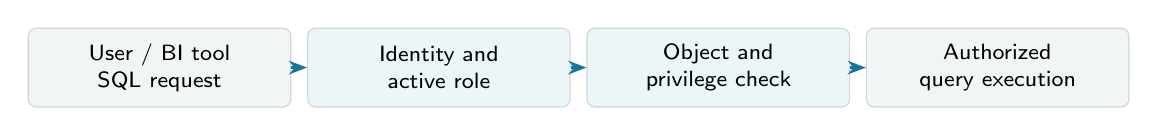
\begin{tikzpicture}[node distance=2mm, every node/.style={font=\sffamily\fontsize{8}{9.8}\selectfont}, b/.style={draw=thinrule,fill=papergray,rounded corners=1mm,minimum height=10mm,text width=31mm,align=center},>=Stealth]
\node[b] (r) {User / BI tool\\SQL request};
\node[b,right=of r,fill=lightblue] (a) {Identity and\\active role};
\node[b,right=of a,fill=lightblue] (c) {Object and\\privilege check};
\node[b,right=of c] (e) {Authorized\\query execution};
\draw[->,thick,steelblue](r)--(a);\draw[->,thick,steelblue](a)--(c);\draw[->,thick,steelblue](c)--(e);
\end{tikzpicture}
\end{center}
{\small\color{inkgray}\textbf{Figure 2.3.} A simplified authorization boundary. Policies and specific object privileges can add checks not shown.}\par

\textbf{An architectural consequence.} Shared data does not imply shared authority. The same storage may serve authorized analysts and transformation engineers while role hierarchies and governance policies constrain access. A secure architecture therefore documents \emph{which identity runs each task}, which role it activates, and the precise privileges needed.

\begin{whitebox}
\textbf{Failure investigation: permission versus performance}\par
An ``insufficient privileges'' error is a configuration or policy issue, not evidence of a slow warehouse. Record the role, intended object, expected access, and observed error. Never solve a tutorial's access problem by casually switching every step to \texttt{ACCOUNTADMIN}.
\end{whitebox}
\textbf{Decision checkpoint.} For a public energy dashboard, a narrow read-only role should see curated aggregates rather than necessarily all raw records. That boundary is more durable than relying on the BI tool to hide restricted columns. Section 13.2 provides role-hierarchy implementation details.

\newpage
% PAGE 26 - 2.4.2
\section*{2.4\quad From SQL to a physical plan}
\topic{2.4.2}{Query compilation, optimization, and metadata}
The SQL text is a request for a result, not a program that dictates each storage access. A query such as ``return the average reported wind power for yesterday'' can be implemented through different physical strategies. Snowflake resolves names and types, validates the expression, considers object metadata and statistics, and constructs an execution plan. Optimization concerns the amount of data to scan, the way operators are arranged, and how work is distributed; the private implementation may change across releases [1,6].

\begin{lstlisting}[language=SQL,caption={A deliberately small, semantically explicit analytical query.}]
SELECT source,
       AVG(power_mw) AS mean_power_mw
FROM BOOK_DEV.CH02_LAB.ENERGY_READING
WHERE event_utc >= '2026-01-15'::TIMESTAMP_NTZ
  AND event_utc <  '2026-01-16'::TIMESTAMP_NTZ
GROUP BY source;
\end{lstlisting}
This is \emph{not} meaningful energy in MWh. An arithmetic average of MW readings becomes a valid measure of mean power only when sampling semantics support the calculation. Unequal intervals or missing samples require explicit weighting and completeness rules. The distinction carries forward from Chapter 1.

\textbf{Conceptual execution path:}
\begin{enumerate}
\item Resolve the database, schema, table, and the active session context.
\item Confirm privileges and determine whether an eligible persisted result can be reused.
\item If the query requires execution, compile and optimize operators using metadata and constraints.
\item Execute the plan, scan required columns and partitions, aggregate, and return results.
\item Record execution activity that authorized users can inspect through Query History and Query Profile.
\end{enumerate}

\begin{insight}
\textbf{Why selectivity is architectural}\par
A precise date range may let metadata eliminate irrelevant micro-partitions before their bytes reach the query operators. This is a storage-organizational advantage expressed through the query plan. A faster result is therefore not necessarily evidence that the warehouse has become more powerful.
\end{insight}
\textbf{Common misconception.} ``The table has an index on the date.'' Standard Snowflake tables use automated micro-partition organization, not a user-managed B-tree index on each column. Hybrid tables have a different indexed storage engine and serve different workloads [1,11]. \textbf{Common diagnostic mistake.} Calling an optimized query slow based on one run that included resume/compile overhead, while comparing it with a result-cache hit on another run.

\repo{P015: A Simple API Powered by Snowflake}{https://github.com/Snowflake-Labs/sfguide-snowflake-python-api}

\newpage
% PAGE 27 - 2.4.3
\section*{2.4\quad Managed coordination has costs too}
\topic{2.4.3}{Managed services versus user-managed compute}
Snowflake operates the cloud-services layer; the customer does not provision its underlying service machines. That does not mean coordination work is economically irrelevant. Metadata queries, compilation, access-control checks, and other services still consume platform resources and may contribute to cloud-services billing under the account's current terms. Compute charges for virtual warehouses, serverless features, data storage, and transfers are distinct cost categories [1,10].

A useful distinction is between \emph{what the engineer configures} and \emph{what the engineer operates}. You select warehouse sizes and choose SQL/data models; Snowflake maintains much of the underlying infrastructure and query service. Your team remains accountable for query semantics, role design, observability, recoverability, and the bill resulting from the architecture.

\begin{center}\small
\begin{tabularx}{\linewidth}{@{}p{29mm}X X@{}}\toprule
\textbf{Concern} & \textbf{Managed by platform} & \textbf{Owner's decision}\\\midrule
Persistent layout & Micro-partition encoding and metadata & Data model, table type, load pattern\\
Query planning & Parsing and optimization services & SQL semantics, filters, workload tests\\
Execution capacity & Warehouse infrastructure & Warehouse selection, size, suspend policy\\
Authorization & Role/privilege enforcement & Least-privilege design and assignments\\
Recovery & Supported retention mechanisms & Retention choice, backup and incident plan\\
\bottomrule\end{tabularx}\end{center}

\textbf{A practical governance scenario.} The Finland Energy Analytics project is run by one data engineer but read by many BI users. It is tempting to use a single high-privilege role for every script and dashboard. A better model assigns a deployment role to create approved objects, a transformation role to write curated tables, and a reporting role that reads only the required outputs. The specific grants must be tested later; what matters here is the boundary between responsibilities.

\textbf{Cost reasoning.} For a new job, record the number of calls, query durations, warehouse uptime, bytes transferred, and any use of managed serverless functionality. A \emph{credit-per-query} estimate is incomplete when other billable services also contribute. No static USD-per-credit value should be treated as universal across regions and contracts.

\begin{whitebox}
\textbf{Small architecture exercise}\par
An analyst receives a permissions error, another user sees a ten-second warehouse resume delay, and a third user sees a three-second table scan. Assign each event to its primary layer and propose one observation that would confirm your diagnosis. The three cases require different remedies, even though every user describes the dashboard as ``not working.''
\end{whitebox}
\repo{P016: Getting Started with the Snowflake Python API}{https://github.com/Snowflake-Labs/sfguide-getting-started-snowflake-python-api}

\newpage
% PAGE 28 - 2.5.1
\section*{2.5\quad Query pruning, caching, and data access}
\topic{2.5.1}{Micro-partition pruning}
The cheapest byte to process is often the byte never read. When a filter narrows the requested time range, Snowflake can use metadata to exclude micro-partitions that could not contain qualifying values. This is \emph{pruning}. It differs from filtering rows \emph{after} scanning: both can produce the correct answer, but the number of partitions read may differ substantially. Query Profile exposes TableScan statistics, including \emph{Partitions scanned} and \emph{Partitions total}, that help diagnose the difference [2,6].

\begin{center}\small
\begin{tabularx}{\linewidth}{@{}p{45mm}X@{}}\toprule
\textbf{Illustrative metric} & \textbf{Interpreting the observation}\\\midrule
Scanned 12 of 1,200 partitions & Strong candidate for effective pruning; confirm query and bytes\\
Scanned 1,175 of 1,200 & Filter eliminated little stored data; investigate necessity and layout\\
Scanned 0; returned instantly & May represent result reuse; verify rather than infer a fast scan\\
\bottomrule\end{tabularx}\end{center}

Those counts are made-up \emph{examples}, not measured Snowflake outputs. Define a pruning ratio as \(r=\text{scanned}/\text{total}\) only when total is nonzero. A lower ratio may be desirable for selective queries; it is not an overall performance score. One query may scan nearly every partition because the business genuinely asked for all history.

\textbf{A predicate experiment.} In an isolated test table containing many days of readings, compare a bounded UTC interval with a query for the entire table. Keep projection, warehouse, and session conditions as stable as practicable. Make sure the result is not served from a previously persisted result; then inspect the TableScan metrics. Do not extrapolate a large-data performance claim from a ten-row classroom table.

\begin{lstlisting}[language=SQL,caption={An explicit half-open UTC interval predicate.}]
WHERE event_utc >= '2026-01-01'::TIMESTAMP_NTZ
  AND event_utc <  '2026-02-01'::TIMESTAMP_NTZ
\end{lstlisting}

A half-open interval has a clear boundary, avoids constructing a last millisecond, and works naturally across adjacent periods. Its semantics still depend on storing and interpreting timestamps consistently: \texttt{TIMESTAMP\_NTZ} does not itself carry a time-zone offset. Preserve the chosen UTC convention in the data contract.

\textbf{Failure mode.} Declare clustering keys without validating selectivity, write patterns, or maintenance cost. Begin with the workload: identify common filters and joins, then decide whether physical reorganization is justified.
\repo{P017: Query Performance Deep-Dive}{https://github.com/sfc-gh-bokon/query_performance_deep_dive}

\newpage
% PAGE 29 - 2.5.2
\section*{2.5\quad Three different meanings of cache}
\topic{2.5.2}{Result reuse and data/cache behavior}
Snowflake users often say, ``The second query is faster because it is cached,'' but several distinct effects can produce shorter response time. \emph{Persisted query-result reuse} can return an eligible prior result without repeating execution. Separately, \emph{warehouse data caching} can retain frequently used data on an active warehouse's local resources, reducing future remote reads. Finally, query compilation, initialization, and system load can vary between runs even without a cache hit [3,5].

\begin{center}\small
\begin{tabularx}{\linewidth}{@{}p{30mm}X X@{}}\toprule
\textbf{Mechanism} & \textbf{What is reused?} & \textbf{Investigation question}\\\midrule
Persisted result & Final earlier query result, when eligible & Did the query actually execute?\\
Warehouse cache & Accessed data on local warehouse resources & Was remote I/O reduced?\\
Plan and runtime state & Compilation/runtime conditions can vary & Were startup and workloads comparable?\\
\bottomrule\end{tabularx}\end{center}

Snowflake documents a normal 24-hour lifetime for persisted query results, subject to eligibility and reuse behavior; this is not a promise that every repeated query will hit the cache. Data changes, mismatched SQL text, permissions, non-reusable functions, and other conditions can defeat reuse [5]. A suspended warehouse may lose some or all useful local cache; consequently aggressive suspension can save credits but also alter performance. Neither rule justifies a universal recommendation without observing the workload.

\begin{lstlisting}[language=SQL,caption={Session-level control for a diagnostic, not a speed guarantee.}]
ALTER SESSION SET USE_CACHED_RESULT = FALSE;
-- Run the target SELECT and inspect Query Profile.
-- Then restore the usual behavior:
ALTER SESSION SET USE_CACHED_RESULT = TRUE;
\end{lstlisting}

\textbf{Why this matters.} If the first execution takes 8 seconds and the next returns a previously persisted result in 0.2 seconds, the engineer has not demonstrated a 40-fold improvement in the query plan. The second execution may have bypassed the physical scan altogether. A fair benchmark labels which observations include cached results and which are actual executions.

\begin{insight}
\textbf{Rule of evidence}\par
A successful cache hit demonstrates effective result reuse for that request. It does not prove the underlying table organization, join strategy, or warehouse size is efficient for \emph{new} queries.
\end{insight}
\textbf{Failure mode.} Citing the existence of a cached result as an explanation for correctness. Caches must respect Snowflake's reuse and authorization conditions, but metric correctness still depends on the pipeline and data contract.

\newpage
% PAGE 30 - 2.5.3
\section*{2.5\quad Designing a fair query experiment}
\topic{2.5.3}{Cache misses and fair comparisons}
A performance experiment starts with one hypothesis, not a collection of buttons to press. For the Finland Energy Analytics workload, consider this testable statement: \emph{a selective half-open timestamp predicate scans fewer partitions than the unbounded monthly aggregate on the same fixed dataset}. The observation is a partition count and scanned data volume; elapsed time is secondary until overhead and warehouse conditions have been controlled.

\textbf{Experimental protocol:}
\begin{enumerate}
\item Freeze or document dataset version, row count, timestamp grain, and table type.
\item Record account cloud/region, edition, warehouse size, query text, role, and query tag.
\item Use a dedicated test workload or note concurrent queries; disable persisted-result reuse for the specific diagnostic.
\item Repeat each query enough times to identify obvious outliers; keep warm and cold conditions separately labelled.
\item Inspect scanned/total partitions, bytes read, spill behavior, elapsed time, and queueing.
\item Confirm both queries deliver the correct \emph{intended} answers before interpreting speed.
\end{enumerate}

\begin{whitebox}
\textbf{Correctness comes first.} If one query computes average MW for 24 equal intervals and another computes sum of MW, their execution time is not a fair benchmark because their answers mean different things. Likewise, using UTC in one query and Finnish local time in another may change which intervals belong to the reporting day.
\end{whitebox}

\begin{center}\small
\begin{tabularx}{\linewidth}{@{}p{37mm}X@{}}\toprule
\textbf{Log field} & \textbf{Why keep it?}\\\midrule
\texttt{query\_id}, UTC run time & Locate the exact history and profile\\
SQL hash / saved query & Establish that comparison text is controlled\\
Warehouse, size, cache state & Separate execution effects from environment effects\\
Partitions scanned / total & Quantify pruning for scans with relevant operators\\
Runtime and queue wait & Distinguish CPU/I/O work from capacity contention\\
Result checksum or invariant & Verify correctness independently of latency\\
\bottomrule\end{tabularx}\end{center}

A table with 800 rows may not have enough micro-partitions to show a useful pruning contrast. \emph{A small laboratory is valuable for validating SQL behavior, not for establishing production performance.} A larger representative dataset and an isolated account are needed for meaningful optimization conclusions.

\textbf{Diagnostic outcome.} If both runs have low queue time but scan almost all partitions, add compute only after investigating data organization and filter usefulness. If pruning is efficient but one join spills to remote disk, examine warehouse memory and join strategy. If execution is short but elapsed time includes long queueing, consider workload isolation or concurrency capacity.


\newpage
% PAGE 31 - 2.6
\section*{2.6\quad Concurrency and multi-cluster warehouses}
\topic{2.6.1}{Queueing and throughput under concurrency}
A slow report can mean either \emph{the query itself executes slowly} or \emph{the query waits to begin}. Consider a classroom example: one warehouse can complete a particular analytical request in two seconds, but thirty users submit requests in a short burst. Finite execution slots mean some requests may queue, and end-to-end latency rises although an individual scan remains efficient. Capacity and scheduling must be measured instead of inferred from concurrent user count alone.

\topic{2.6.2}{Multi-cluster use cases and edition limits}
Multi-cluster warehouses can add compute clusters dynamically or use a fixed number of clusters to handle many concurrent requests. The feature requires Enterprise Edition or higher under the documented availability model [4]. Auto-scale policies balance faster response under load against extra credits. A sensible approach is to monitor queueing, reduce expensive or unnecessary requests, isolate workloads if appropriate, and then validate whether additional clusters improve the service-level objective.

\begin{center}
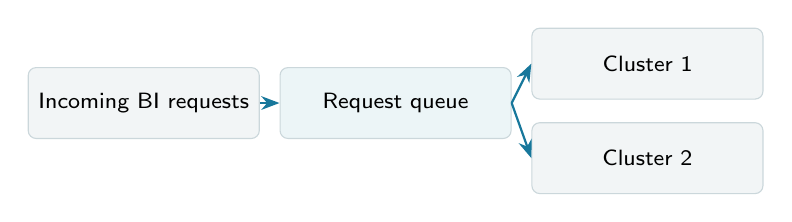
\begin{tikzpicture}[node distance=2.5mm,every node/.style={font=\sffamily\fontsize{8}{9.5}\selectfont},b/.style={draw=thinrule,rounded corners=1mm,fill=papergray,align=center,minimum height=9mm,text width=27mm},>=Stealth]
\node[b] (q) {Incoming BI requests};
\node[b,right=of q,fill=lightblue] (queue) {Request queue};
\node[b,right=of queue,yshift=5mm] (c1) {Cluster 1};
\node[b,right=of queue,yshift=-7mm] (c2) {Cluster 2};
\draw[->,thick,steelblue] (q)--(queue);
\draw[->,thick,steelblue] (queue.east)--(c1.west);
\draw[->,thick,steelblue] (queue.east)--(c2.west);
\end{tikzpicture}
\end{center}
{\small\color{inkgray}\textbf{Figure 2.4.} Conceptual distribution under concurrent load. A multi-cluster warehouse helps process \emph{more requests}; it is not an automatic acceleration of one request.}\par

\topic{2.6.3}{Why more clusters do not guarantee faster single queries}
If one large aggregation is CPU- or memory-bound, making \emph{its assigned cluster} larger may help. Adding another cluster generally addresses simultaneous requests instead. Even scale-up can plateau if the request is restricted by poor pruning, network I/O, skew, or the available parallelism. Record at least median latency, tail latency, queueing, concurrency, and credits for the actual workload before and after change.

\begin{insight}
\textbf{Scale the identified bottleneck}\par
\emph{More memory and CPU per cluster} may help a demanding single query. \emph{More clusters} may help concurrency. \emph{Better pruning or SQL} may reduce work for every cluster. These are competing investments, not synonyms.
\end{insight}
\textbf{Failure mode.} Compare a busy weekday on a single cluster with a quiet Sunday on a multi-cluster setup and attribute the difference solely to the cluster count. Without controlled concurrency and cost, this is not convincing evidence.
\repo{P018: Snowpark Python Performance Guide}{https://github.com/Snowflake-Labs/sfguide-snowpark-python-top-three-tips-for-optimal-performance}

\newpage
% PAGE 32 - 2.7.1
\section*{2.7\quad Time Travel, Fail-safe, and data retention}
\topic{2.7.1}{Time Travel recovery paths}
Storage architecture is also a recovery decision. If a transformation accidentally overwrites a table at noon, can the team inspect the previous state and restore it? Snowflake Time Travel can expose historical versions within an applicable retention window, including supported recovery operations on database objects. It is designed for \emph{user-accessible historical querying and recovery}, not as a substitute for a complete backup, replication, or disaster-recovery strategy [7].

In the energy project, imagine that one daily load mistakenly interpreted missing values as zero. A query of the prior table state can help diagnose the change if that history remains inside the configured window. The responsible engineer should first pause the faulty process, identify the relevant change time or statement, and validate the historical result before restoring or copying data.

\begin{lstlisting}[language=SQL,caption={A read-only historical query; an eligible table and retention window are required.}]
-- Example only: inspect a table's prior state.
SELECT COUNT(*) AS row_count_before_change
FROM BOOK_DEV.CH02_LAB.ENERGY_READING
  AT (OFFSET => -60 * 30);
\end{lstlisting}

The example requests a point approximately thirty minutes earlier. Its success depends on current retention, privileges, object type, and the table's history. It is not executed in this manuscript, and the existence of an earlier version must not be assumed. A recovery operation should be rehearsed on test objects before being applied to production data.

\begin{center}\small
\begin{tabularx}{\linewidth}{@{}p{38mm}X@{}}\toprule
\textbf{Recovery question} & \textbf{Evidence required}\\\midrule
When did wrong data appear? & Load/job history and first incorrect output\\
What was the last correct state? & Time Travel query or trusted source snapshot\\
What else changed after that? & Downstream writes, consumers, and dependencies\\
Can we recover safely? & Retention availability, restore plan, validation tests\\
\bottomrule\end{tabularx}\end{center}

\textbf{Recovery principle.} An impressive \texttt{UNDROP} command does not guarantee restoration of every business outcome. Materialized reports, external consumers, cached extracts, and downstream updates may need separate correction. Runbooks should define owners, communication, and repeatable validation.

\newpage
% PAGE 33 - 2.7.2 2.7.3
\section*{2.7\quad Retention is a design parameter}
\topic{2.7.2}{Fail-safe scope and operational boundaries}
Fail-safe and Time Travel solve different problems. Time Travel is a customer-facing historical access feature inside configured limits. Fail-safe is a Snowflake-operated recovery mechanism for eligible permanent-table history after Time Travel, with a seven-day period; it is not an ordinary query interface or an on-demand replacement for Time Travel. Snowflake Support involvement and recovery scope differ from self-service restoration [7,8].

\topic{2.7.3}{Retention choices by object type and edition}
Under documented standard-table behavior, permanent tables have a seven-day Fail-safe period. Standard Edition generally supports a one-day Time Travel period; Enterprise Edition and above permit eligible longer retention, up to 90 days. Transient and temporary tables have at most one day of Time Travel and no Fail-safe; temporary-table lifetime is also tied to session behavior [7,8]. These rules have object-type and feature-specific exceptions, so check the current documentation for the specific asset before relying on a retention number.

\begin{center}\small
\begin{tabularx}{\linewidth}{@{}p{29mm}p{32mm}X@{}}\toprule
\textbf{Table category} & \textbf{Time Travel (typical)} & \textbf{Fail-safe / caution}\\\midrule
Permanent, Standard & 0--1 day configured & 7 days; historical storage may be billed\\
Permanent, Enterprise+ & 0--90 days when supported & 7 days; longer history increases storage exposure\\
Transient & 0--1 day & No Fail-safe; unsuitable as only protection for valuable data\\
Temporary & 0--1 day while eligible & No Fail-safe; session lifecycle constrains recovery\\
\bottomrule\end{tabularx}\end{center}

\textbf{Retention has an economic dimension.} Old versions and deleted data can consume storage. Selecting the longest permitted period for every large intermediate table is not necessarily the safest or most economical architecture. Choose retention according to recovery-point requirements, ability to recreate data from source, legal obligations, and storage cost [8].

\begin{whitebox}
\textbf{Incident design exercise}\par
A curated daily metric table must be recoverable after accidental modification discovered three days later. A one-day Time Travel policy alone does not satisfy that user-accessible recovery requirement. Propose a supported longer-retention option when eligible, plus source snapshots or another recovery mechanism and a tested process. State which options depend on account edition.
\end{whitebox}

\textbf{Failure mode.} Calling Fail-safe a standard self-service backup; choosing transient raw tables without ensuring the raw files can be replayed; assuming an Iceberg table stored outside Snowflake has exactly the same protection as a permanent native table.
\repo{P019: Time-Travel Table dbt Package}{https://github.com/edx/snowflake_timetravel_table}

\newpage
% PAGE 34 - 2.8.1,2.8.2
\section*{2.8\quad Cloud regions, deployment models, and limitations}
\topic{2.8.1}{Cloud provider, deployment region, and data residency}
A Snowflake account resides in a selected cloud-provider region. That decision affects available capabilities, latency to producers and consumers, data movement, resilience options, and applicable organizational or legal constraints. \emph{Data residency} is not established merely by writing the word ``Finland'' in a schema name. The engineer must identify where bytes are stored, where computations run, which connected services receive information, and whether replication or external integrations cross borders [9,10].

For a Finland-based publisher's example project, the geographical name refers to the \emph{subject of the measurements}; it does not guarantee the data is hosted in Finland. A realistic architecture record separately states: source-system region, Snowflake account region, external storage location, BI user regions, and any cross-region processing. For personal or regulated data, the choice must be assessed against applicable policies and legal obligations; public energy data may have different constraints.

\topic{2.8.2}{Availability differences across regions}
The name ``Snowflake'' does not guarantee every table type, external integration, model, or AI feature is usable in every account. Features may depend on cloud, region, edition, preview enrollment, or contract. For example, Snowflake's published limitations describe hybrid-table availability in commercial AWS and Azure regions, with restrictions for other environments and trial accounts [11]. Such boundaries are subject to change and need a dated check when the book is finalized.

\begin{center}\small
\begin{tabularx}{\linewidth}{@{}p{35mm}X@{}}\toprule
\textbf{Deployment decision} & \textbf{Questions to record}\\\midrule
Region and provider & Where must data reside; where are users and source systems?\\
Edition and access & Does the exact feature exist for this account and role?\\
External integrations & Which credentials, endpoints, regions, and trust boundaries?\\
Continuity design & Which region failure must be tolerated; what recovery objectives?\\
\bottomrule\end{tabularx}\end{center}

\begin{insight}
\textbf{A useful design rule}\par
Write the region/edition compatibility matrix \emph{before} choosing a critical feature. A hands-on book must never require an unavailable feature without offering a lower-cost, region-compatible fallback.
\end{insight}
\textbf{Failure mode.} Replicate data to a different region to improve availability without checking who is allowed to receive the data, how it will be recovered, and what recurring transfer costs arise.
\repo{P020: Snowflake MCP and Bedrock AgentCore Guide}{https://github.com/Snowflake-Labs/sfguide-getting-started-with-snowflake-managed-mcp-and-bedrock-agentcore}

\newpage
% PAGE 35 - 2.8.3
\section*{2.8\quad Locality, transfer, and environment separation}
\topic{2.8.3}{Data transfer costs and environment separation}
Moving data between services is not always a zero-cost internal operation. Compute in Snowflake may be billed separately from storage and from relevant network or cross-region transfer activities. When Iceberg tables use external volumes, costs and responsibilities depend on who owns the storage, what crosses cloud or region boundaries, and which engine reads or writes files [9,12]. Always consult current documentation and account terms instead of treating one provider's example cost as a universal tariff.

\textbf{Example: a cross-region architecture.} A source system writes Parquet files to a cloud bucket in Region A. Snowflake computes in Region B while BI users are mainly in Region C. The analyst sees only a table; the engineering team must examine three different kinds of locality: data-location and access permissions, physical transfer flows, and the placement of compute. Moving the BI endpoint alone will not necessarily remove storage transfer costs.

\begin{center}

\begin{tikzpicture}[every node/.style={font=\sffamily\fontsize{8}{9.8}\selectfont},b/.style={draw=thinrule,rounded corners=1mm,fill=papergray,text width=37mm,minimum height=12mm,align=center},>=Stealth]
\node[b] (a) {Region A\\ Source files / API};
\node[b,right=6mm of a,fill=lightblue] (b) {Region B\\ Snowflake account};
\node[b,right=6mm of b] (c) {Region C\\ BI consumers};
\draw[->,thick,steelblue] (a)--node[above,font=\sffamily\fontsize{7.4}{8.5}\selectfont]{transfer?}(b);
\draw[->,thick,steelblue] (b)--node[above,font=\sffamily\fontsize{7.4}{8.5}\selectfont]{results}(c);
\end{tikzpicture}
\end{center}
{\small\color{inkgray}\textbf{Figure 2.5.} A conceptual regional dependency map. Charges and restrictions vary with operation and service; not every arrow incurs the same Snowflake fee.}\par

\textbf{Separate environments.} Development, test, and production should not share unrestricted operational authority merely for convenience. Physical separation might use schemas, databases, separate warehouses, accounts, or more than one of these. The appropriate level follows the sensitivity and blast-radius requirements. A learning lab should never overwrite production objects because a default database happened to be selected.

\textbf{Energy capstone checks:}
\begin{enumerate}
\item Are we using only public, correctly licensed inputs or any identifiable operational data?
\item Where do each source, managed table, optional external volume, and dashboard operate?
\item Can this run in a sandbox without unexpected service charges?
\end{enumerate}

\begin{whitebox}
\textbf{Deployment evidence to retain}\par
Cloud/provider/region; feature availability; least-privilege connectivity; source and destination locations; data-reuse license; cross-border processing; expected credit, storage, and network categories; account configuration and date checked.
\end{whitebox}
\repo{P021: Openflow Deployment Guide}{https://github.com/Snowflake-Labs/sfguide-getting-started-with-openflow-spcs}

\newpage
% PAGE 36 - 2.9
\section*{2.9\quad Reference architectures and design trade-offs}
\topic{2.9.1}{Batch-first versus streaming designs}
A well-designed architecture is proportional to its requirements. For a validated daily electricity report, scheduled file/API ingestion and an incremental transformation may be sufficient. A near-live operations screen might justify a different ingestion approach. Neither choice is inherently superior: freshness, replay, observability, error recovery, and cost must be considered together. Do not choose a stream merely to make the architecture diagram look modern.

\topic{2.9.2}{Snowflake-managed versus external storage}
Standard Snowflake tables use platform-managed columnar micro-partitions. Iceberg tables adopt an open table format and can be backed by Snowflake-managed storage or by customer-managed external volumes, with responsibility and recovery differences. External files may make multi-engine integration attractive but also introduce catalog, access, lifecycle, and egress questions. Evaluate the \emph{whole operating model}, not only the nominal storage price [1,12].

\topic{2.9.3}{Native, Iceberg, and hybrid table considerations}
Hybrid tables use an indexed row-oriented engine for low-latency reads and writes and have different feature/region limitations. They should not be marketed as drop-in replacements for scan-optimized analytical tables. Conversely, open table formats may be valuable where portability and interoperability matter more than tightly integrated managed behavior [1,11,12].

\begin{center}\small
\begin{tabularx}{\linewidth}{@{}p{23mm}X X@{}}\toprule
\textbf{Choice} & \textbf{Good first reason} & \textbf{Main design caution}\\\midrule
Standard Snowflake table & Managed SQL analytics and transformation & Proprietary storage organization; compute/cost model\\
Iceberg table & Open-format or external-lake interoperability & Catalog/storage ownership and feature scope\\
Hybrid table & Indexed operational reads/writes & Region/edition, workload fit, operational limitations\\
\bottomrule\end{tabularx}\end{center}

\begin{insight}
\textbf{Reference decision for the capstone}\par
Use a \emph{batch-first, managed standard-table architecture} as the starting hypothesis for the Finland Energy Analytics Platform. Keep raw-source provenance and a reproducible transformation path. Treat streaming, external Iceberg storage, and hybrid tables as alternatives to be justified by new requirements, not mandatory components of a basic energy dashboard.
\end{insight}

\textbf{Trade-off checkpoint.} The recommended baseline minimizes deployment dependencies and leaves room to test BI performance. It is not a proof that this architecture is globally cheapest or fastest. The exact API source, daily interval counts, regional setup, licensing, and cost must be determined before implementation.
\repo{P002: Snowflake Iceberg Tables Guide}{https://github.com/Snowflake-Labs/sfguide-getting-started-with-iceberg-tables}
\repo{P022: Data Application with Hybrid Tables}{https://github.com/Snowflake-Labs/sfguide-build-data-application-with-hybrid-tables}

\newpage
% PAGE 37 - LAB
\section*{2.L\quad Guided lab: follow an analytical query}
\topic{2.L.1}{Prerequisites, permissions, and cost controls}
\textbf{Goal.} Draw the capstone's architecture and inspect a Snowflake Query Profile \emph{if} an authorized training account exists. The offline route needs only a text editor and the chapter's supplied data contract; the optional SQL route uses a dedicated test role, an existing X-Small training warehouse, and a new throwaway schema. Never run the SQL against a production database or with broad default privileges.

\begin{whitebox}
\textbf{Cost and security checkpoint}\par
Ask an administrator to provide a sandbox database and a role authorized for schema and table creation only within it. Confirm current warehouse auto-suspend and account cost alerts. End the experiment by suspending the training warehouse if your role and shared-user policy allow it. No hard-coded password, API key, personal data, or customer dataset is required.
\end{whitebox}

\topic{2.L.2}{Step-by-step procedure and a bounded sample query}
\textbf{Offline path.} Copy the conceptual architecture in Figure 2.1 to \texttt{architecture\_v1.svg}. Add an external source, UTC validation and quality gate, a raw table, a curated summary table, and a BI reader. Label separate BI/ELT warehouses as \emph{proposed}, identify each trust boundary, and annotate which layer owns metadata, persistence, and query execution.

\textbf{Optional Snowflake path.} In an approved development database, run the companion SQL script after filling in safe identifiers. It uses a small synthetic \texttt{ENERGY\_READING} table with a known UTC day, and produces counts and aggregates for a query you can find in Query History. The extract below is a representative core, not an assertion of observed execution.

\begin{lstlisting}[language=SQL,caption={Core of the optional teaching query; synthetic records only.}]
ALTER SESSION SET QUERY_TAG = 'BOOK_CH02_LAB';
ALTER SESSION SET USE_CACHED_RESULT = FALSE;
SELECT source, COUNT(*) AS intervals,
       ROUND(AVG(power_mw), 1) AS mean_power_mw
FROM BOOK_DEV.CH02_LAB.ENERGY_READING
WHERE event_utc >= '2026-01-15'::TIMESTAMP_NTZ
  AND event_utc <  '2026-01-16'::TIMESTAMP_NTZ
GROUP BY source ORDER BY source;
\end{lstlisting}

Locate the statement in \emph{Query History} using the session or query tag, open \emph{Query Profile}, and record the Query ID, execution time, queue time, warehouse, any TableScan, partitions scanned/total, and cache status where displayed. A tiny test table may not show useful pruning: that absence is an expected limit of the lab, not a failure.

\textbf{Deliverables.} Architecture SVG, SQL script, and \texttt{tradeoffs.md}.\par The companion README explains setup, cleanup, and expected output.

\newpage
% PAGE 38 - LAB CONTINUES
\section*{2.L\quad Validate, decide, and review}
\topic{2.L.3}{Expected results, limitations, and cleanup}
For the companion's four illustrative fifteen-minute interval readings, the expected row counts are \texttt{SOLAR=2} and \texttt{WIND=2}, with mean powers \texttt{SOLAR=0.0 MW} and \texttt{WIND=490.0 MW}. These values follow from the \emph{synthetic} rows; they are not observations from a live Snowflake run. The query is not intended to estimate total national electricity production. Query-profile timing, partitions scanned, and total credits are \emph{unknown until your actual lab runs}; never replace them with invented screenshots.

If setup fails, record the error and active role; do not elevate privileges without authorization. If a requested object already exists, stop and check ownership rather than overwrite it. Restore \texttt{USE\_CACHED\_RESULT}, clear the query tag if appropriate, and remove only objects that the lab created in its dedicated namespace. In a shared account, obtain approval before warehouse suspension or teardown.

\topic{2.L.4}{Exercises and scoring rubric}
\textbf{Foundation:} label the storage, compute, and service responsibilities in a query path. \textbf{Practitioner:} describe why one cached run cannot establish an optimization claim; write a controlled comparison plan. \textbf{Production design:} evaluate whether to separate BI and ELT compute for thirty users and a nightly transformation, including cost and recovery risks.

\begin{whitebox}
\textbf{Acceptance checklist and rubric}\par
\begin{itemize}
\item \textbf{Layer model (25\%):} the diagram assigns responsibilities correctly and marks trust boundaries.
\item \textbf{Evidence (25\%):} Query ID and relevant metrics are recorded or explicitly marked not run.
\item \textbf{Decision quality (25\%):} the ADR compares at least two plausible options and names constraints.
\item \textbf{Safety and honesty (25\%):} no credentials or claimed measurements without tests; cleanup is bounded.
\end{itemize}
\end{whitebox}

\textbf{Chapter summary.} Persistent storage organization, execution capacity, and managed cloud services cooperate but address different problems. Query Profile guides changes; cache and queue effects must be separated; recovery retention and region/edition limits shape architecture. The correct answer is not \emph{always use more compute}, but \emph{identify the controlling constraint and document why the selected design fits}.

{\small\sffamily\bfseries\color{steelblue}SELECTED TECHNICAL REFERENCES (DOCUMENTATION CHECK: OCTOBER 2026)}\par
{\fontsize{7.7}{9.2}\selectfont\setstretch{1.0}
[1] Snowflake, \href{https://docs.snowflake.com/en/user-guide/intro-key-concepts}{Key Concepts and Architecture}.\quad
[2] \href{https://docs.snowflake.com/en/user-guide/tables-clustering-micropartitions}{Micro-partitions and Clustering}.\par
[3] \href{https://docs.snowflake.com/en/user-guide/warehouses-considerations}{Warehouse Considerations}.\quad
[4] \href{https://docs.snowflake.com/en/user-guide/warehouses-multicluster}{Multi-cluster Warehouses}.\par
[5] \href{https://docs.snowflake.com/en/user-guide/querying-persisted-results}{Persisted Query Results}.\quad
[6] \href{https://docs.snowflake.com/en/user-guide/ui-snowsight-activity}{Query History and Profile}.\par
[7] \href{https://docs.snowflake.com/en/user-guide/data-availability}{Time Travel and Fail-safe}.\quad
[8] \href{https://docs.snowflake.com/en/user-guide/data-cdp-storage-costs}{Historical Storage Costs}.\par
[9] \href{https://docs.snowflake.com/en/user-guide/secure-data-sharing-across-regions-platforms}{Cross-region Data Sharing}.\quad
[10] \href{https://docs.snowflake.com/en/user-guide/cost-understanding-data-transfer}{Data Transfer Costs}.\par
[11] \href{https://docs.snowflake.com/en/user-guide/tables-hybrid-limitations}{Hybrid Table Limitations}.\quad
[12] \href{https://docs.snowflake.com/en/user-guide/tables-iceberg}{Apache Iceberg Tables}.\par

\end{document}
